\chapter{Phylogenetics with Bio.Phylo}
\label{sec:Phylo}

The Bio.Phylo module was introduced in Biopython 1.54. Following the lead of SeqIO and AlignIO,
it aims to provide a common way to work with phylogenetic trees independently of the source data
format, as well as a consistent API for I/O operations.

Bio.Phylo is described in an open-access journal article \cite[Talevich
\textit{et al.}, 2012]{talevich2012}, which you might also find helpful.

\section{Demo: What's in a Tree?}

To get acquainted with the module, let's start with a tree that we've already constructed, and
inspect it a few different ways.  Then we'll colorize the branches, to use a special phyloXML
feature, and finally save it.

Create a simple Newick file named \texttt{simple.dnd} using your favorite text editor,
or use \href{http://biopython.org/SRC/biopython/Doc/examples/simple.dnd}{\texttt{simple.dnd}}
provided with the Biopython source code:

\begin{verbatim}
(((A,B),(C,D)),(E,F,G));
\end{verbatim}

This tree has no branch lengths, only a topology and labelled terminals. (If you have a real
tree file available, you can follow this demo using that instead.)

Launch the Python interpreter of your choice:

\begin{verbatim}
% ipython -pylab
\end{verbatim}

For interactive work, launching the IPython interpreter with the \verb|-pylab| flag enables
\textbf{matplotlib} integration, so graphics will pop up automatically. We'll use that during
this demo.

Now, within Python, read the tree file, giving the file name and the name of the format.

%doctest examples
\begin{verbatim}
>>> from Bio import Phylo
>>> tree = Phylo.read("simple.dnd", "newick")
\end{verbatim}

Printing the tree object as a string gives us a look at the entire object hierarchy.

%cont-doctest
\begin{verbatim}
>>> print(tree)
Tree(rooted=False, weight=1.0)
    Clade()
        Clade()
            Clade()
                Clade(name='A')
                Clade(name='B')
            Clade()
                Clade(name='C')
                Clade(name='D')
        Clade()
            Clade(name='E')
            Clade(name='F')
            Clade(name='G')
\end{verbatim}

The \texttt{Tree} object contains global information about the tree, such as whether it's
rooted or unrooted. It has one root clade, and under that, it's nested lists of clades all the
way down to the tips.

The function \verb|draw_ascii| creates a simple ASCII-art (plain text) dendrogram.  This is a
convenient visualization for interactive exploration, in case better graphical tools aren't
available.

%doctest examples
\begin{verbatim}
>>> from Bio import Phylo
>>> tree = Phylo.read("simple.dnd", "newick")
>>> Phylo.draw_ascii(tree)
                                                    ________________________ A
                           ________________________|
                          |                        |________________________ B
  ________________________|
 |                        |                         ________________________ C
 |                        |________________________|
_|                                                 |________________________ D
 |
 |                         ________________________ E
 |                        |
 |________________________|________________________ F
                          |
                          |________________________ G
<BLANKLINE>
\end{verbatim}

If you have \textbf{matplotlib} or \textbf{pylab} installed, you can create a graphic
using the \verb|draw| function (see Fig. \ref{fig:phylo-simple-draw}):

\begin{verbatim}
>>> tree.rooted = True
>>> Phylo.draw(tree)
\end{verbatim}

\begin{htmlonly}
\imgsrc[width=666, height=530]{images/phylo-simple-draw.png}
\label{fig:phylo-simple-draw}
\end{htmlonly}

\begin{latexonly}
\begin{figure}[htb]
\centering
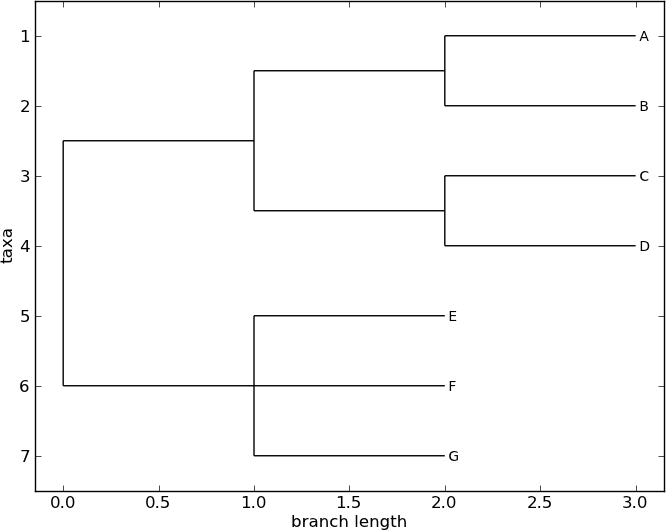
\includegraphics[width=0.7\textwidth]{images/phylo-simple-draw.png}
\caption{A rooted tree drawn with {\tt Phylo.draw}.}
\label{fig:phylo-simple-draw}
\end{figure}
\end{latexonly}


\subsection{Coloring branches within a tree}

The functions \verb|draw| and \verb|draw_graphviz| support the display of different
colors and branch widths in a tree.
As of Biopython 1.59, the \verb|color| and \verb|width| attributes are available on the
basic Clade object and there's nothing extra required to use them.
Both attributes refer to the branch leading the given clade, and apply recursively, so
all descendent branches will also inherit the assigned width and color values during
display.

In earlier versions of Biopython, these were special features of PhyloXML trees, and
using the attributes required first converting the tree to a subclass of the basic tree
object called Phylogeny, from the Bio.Phylo.PhyloXML module.

In Biopython 1.55 and later, this is a convenient tree method:

\begin{verbatim}
>>> tree = tree.as_phyloxml()
\end{verbatim}

In Biopython 1.54, you can accomplish the same thing with one extra import:

\begin{verbatim}
>>> from Bio.Phylo.PhyloXML import Phylogeny
>>> tree = Phylogeny.from_tree(tree)
\end{verbatim}

Note that the file formats Newick and Nexus don't support branch colors or widths, so
if you use these attributes in Bio.Phylo, you will only be able to save the values in
PhyloXML format. (You can still save a tree as Newick or Nexus, but the color and width
values will be skipped in the output file.)

Now we can begin assigning colors.
First, we'll color the root clade gray.  We can do that by assigning the 24-bit color
value as an RGB triple, an HTML-style hex string, or the name of one of the predefined
colors.

\begin{verbatim}
>>> tree.root.color = (128, 128, 128)
\end{verbatim}

Or:

\begin{verbatim}
>>> tree.root.color = "#808080"
\end{verbatim}

Or:

\begin{verbatim}
>>> tree.root.color = "gray"
\end{verbatim}

Colors for a clade are treated as cascading down through the entire clade, so when we colorize
the root here, it turns the whole tree gray.  We can override that by assigning a different
color lower down on the tree.

Let's target the most recent common ancestor (MRCA) of the nodes named ``E'' and ``F''.  The
\verb|common_ancestor| method returns a reference to that clade in the original tree, so when
we color that clade ``salmon'', the color will show up in the original tree.

\begin{verbatim}
>>> mrca = tree.common_ancestor({"name": "E"}, {"name": "F"})
>>> mrca.color = "salmon"
\end{verbatim}

If we happened to know exactly where a certain clade is in the tree, in terms of nested list
entries, we can jump directly to that position in the tree by indexing it.  Here, the index
\verb|[0,1]| refers to the second child of the first child of the root.

\begin{verbatim}
>>> tree.clade[0, 1].color = "blue"
\end{verbatim}

Finally, show our work (see Fig. \ref{fig:phylo-color-draw}):

\begin{verbatim}
>>> Phylo.draw(tree)
\end{verbatim}

\begin{htmlonly}
\imgsrc[width=666, height=530]{images/phylo-color-draw.png}
\label{fig:phylo-color-draw}
\end{htmlonly}

\begin{latexonly}
\begin{figure}[htb]
\centering
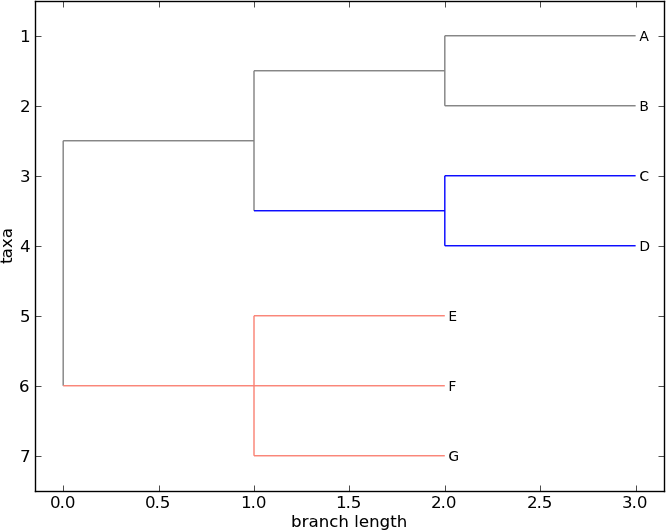
\includegraphics[width=0.7\textwidth]{images/phylo-color-draw.png}
\caption{A colorized tree drawn with {\tt Phylo.draw}.}
\label{fig:phylo-color-draw}
\end{figure}
\end{latexonly}

Note that a clade's color includes the branch leading to that clade, as well as its
descendents. The common ancestor of E and F turns out to be just under the root, and with this
coloring we can see exactly where the root of the tree is.

My, we've accomplished a lot! Let's take a break here and save our work.  Call the
\texttt{write} function with a file name or handle --- here we use standard output, to see what
would be written --- and the format \texttt{phyloxml}.  PhyloXML saves the colors we assigned,
so you can open this phyloXML file in another tree viewer like Archaeopteryx, and the colors
will show up there, too.

\begin{verbatim}
>>> import sys
>>> Phylo.write(tree, sys.stdout, "phyloxml")

<phy:phyloxml xmlns:phy="http://www.phyloxml.org">
  <phy:phylogeny rooted="true">
    <phy:clade>
      <phy:branch_length>1.0</phy:branch_length>
      <phy:color>
        <phy:red>128</phy:red>
        <phy:green>128</phy:green>
        <phy:blue>128</phy:blue>
      </phy:color>
      <phy:clade>
        <phy:branch_length>1.0</phy:branch_length>
        <phy:clade>
          <phy:branch_length>1.0</phy:branch_length>
          <phy:clade>
            <phy:name>A</phy:name>
            ...
\end{verbatim}

The rest of this chapter covers the core functionality of Bio.Phylo in greater detail. For more
examples of using Bio.Phylo, see the cookbook page on Biopython.org:

\url{http://biopython.org/wiki/Phylo_cookbook}

\section{I/O functions}

Like SeqIO and AlignIO, Phylo handles file input and output through four functions:
\verb|parse|, \verb|read|, \verb|write| and \verb|convert|,
all of which support the tree file formats Newick, NEXUS, phyloXML and NeXML, as
well as the Comparative Data Analysis Ontology (CDAO).

The \verb|read| function parses a single tree in the given file and returns it. Careful; it
will raise an error if the file contains more than one tree, or no trees.

\begin{verbatim}
>>> from Bio import Phylo
>>> tree = Phylo.read("Tests/Nexus/int_node_labels.nwk", "newick")
>>> print(tree)
\end{verbatim}

(Example files are available in the \texttt{Tests/Nexus/} and \texttt{Tests/PhyloXML/}
directories of the Biopython distribution.)

To handle multiple (or an unknown number of) trees, use the \verb|parse| function iterates
through each of the trees in the given file:

\begin{verbatim}
>>> trees = Phylo.parse("../../Tests/PhyloXML/phyloxml_examples.xml", "phyloxml")
>>> for tree in trees:
...     print(tree)
\end{verbatim}

Write a tree or iterable of trees back to file with the \verb|write| function:

%cont-doctest
\begin{verbatim}
>>> trees = list(Phylo.parse("../../Tests/PhyloXML/phyloxml_examples.xml", "phyloxml"))
>>> tree1 = trees[0]
>>> others = trees[1:]
>>> Phylo.write(tree1, "tree1.nwk", "newick")
1
>>> Phylo.write(others, "other_trees.nwk", "newick")
12
\end{verbatim}

Convert files between any of the supported formats with the \verb|convert| function:

\begin{verbatim}
>>> Phylo.convert("tree1.nwk", "newick", "tree1.xml", "nexml")
1
>>> Phylo.convert("other_trees.xml", "phyloxml", "other_trees.nex", "nexus")
12
\end{verbatim}

To use strings as input or output instead of actual files, use \verb|StringIO| as you would
with SeqIO and AlignIO:

%doctest
\begin{verbatim}
>>> from Bio import Phylo
>>> from StringIO import StringIO
>>> handle = StringIO("(((A,B),(C,D)),(E,F,G));")
>>> tree = Phylo.read(handle, "newick")
\end{verbatim}


\section{View and export trees}

The simplest way to get an overview of a \verb|Tree| object is to \verb|print| it:

%doctest ../Tests
\begin{verbatim}
>>> from Bio import Phylo
>>> tree = Phylo.read("PhyloXML/example.xml", "phyloxml")
>>> print(tree)
Phylogeny(description='phyloXML allows to use either a "branch_length" attribute...', name='example from Prof. Joe Felsenstein's book "Inferring Phyl...', rooted=True)
    Clade()
        Clade(branch_length=0.06)
            Clade(branch_length=0.102, name='A')
            Clade(branch_length=0.23, name='B')
        Clade(branch_length=0.4, name='C')
\end{verbatim}

This is essentially an outline of the object hierarchy Biopython uses to represent a tree. But
more likely, you'd want to see a drawing of the tree. There are three functions to do this.

As we saw in the demo, \verb|draw_ascii| prints an ascii-art drawing of the tree (a
rooted phylogram) to standard output, or an open file handle if given. Not all of the
available information about the tree is shown, but it provides a way to quickly view the
tree without relying on any external dependencies.

\begin{verbatim}
>>> tree = Phylo.read("example.xml", "phyloxml")
>>> Phylo.draw_ascii(tree)
             __________________ A
  __________|
_|          |___________________________________________ B
 |
 |___________________________________________________________________________ C

\end{verbatim}

The \verb|draw| function draws a more attractive image using the matplotlib
library. See the API documentation for details on the arguments it accepts to
customize the output.

\begin{verbatim}
>>> tree = Phylo.read("example.xml", "phyloxml")
>>> Phylo.draw(tree, branch_labels=lambda c: c.branch_length)
\end{verbatim}

\begin{htmlonly}
\imgsrc[width=701, height=465]{images/phylo-draw-example.png}
\label{fig:phylo-draw-example}
\end{htmlonly}

\begin{latexonly}
\begin{figure}[tbp]
\centering
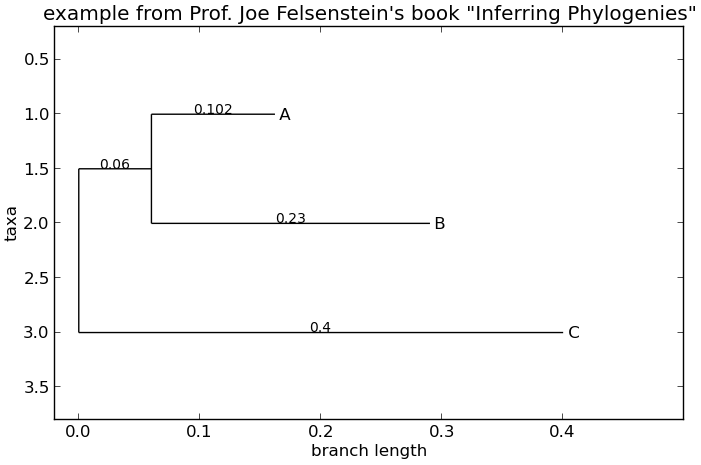
\includegraphics[width=0.7\textwidth]{images/phylo-draw-example.png}
\caption{A simple rooted tree plotted with the {\tt draw} function.}
\label{fig:phylo-draw-example}
\end{figure}
\end{latexonly}


\verb|draw_graphviz| draws an unrooted cladogram, but requires that you have Graphviz,
PyDot or PyGraphviz, NetworkX, and matplotlib (or pylab) installed. Using the same example as
above, and the \verb|dot| program included with Graphviz, let's draw a rooted tree (see
Fig.~\ref{fig:phylo-dot}):

\begin{verbatim}
>>> tree = Phylo.read("example.xml", "phyloxml")
>>> Phylo.draw_graphviz(tree, prog='dot')
>>> import pylab
>>> pylab.show()                    # Displays the tree in an interactive viewer
>>> pylab.savefig('phylo-dot.png')  # Creates a PNG file of the same graphic
\end{verbatim}

\begin{htmlonly}
\imgsrc[width=400, height=312]{images/phylo-dot.png}
\label{fig:phylo-dot}
\end{htmlonly}

\begin{latexonly}
\begin{figure}[tbp]
\centering
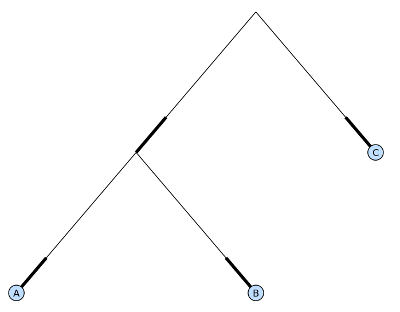
\includegraphics[width=0.5\textwidth]{images/phylo-dot.png}
\caption{A simple rooted tree drawn with {\tt draw\_graphviz}, using {\tt dot} for node
layout.}
\label{fig:phylo-dot}
\end{figure}
\end{latexonly}

(Tip: If you execute IPython with the \verb|-pylab| option, calling \verb|draw_graphviz| causes
the matplotlib viewer to launch automatically without manually calling \verb|show()|.)

This exports the tree object to a NetworkX graph, uses Graphviz to lay out the nodes, and
displays it using matplotlib.
There are a number of keyword arguments that can modify the resulting diagram, including
most of those accepted by the NetworkX functions \verb|networkx.draw| and
\verb|networkx.draw_graphviz|.

The display is also affected by the \verb|rooted| attribute of the given tree object.
Rooted trees are shown with a ``head'' on each branch indicating direction (see
Fig.~\ref{fig:phylo-rooted}):

\begin{verbatim}
>>> tree = Phylo.read("simple.dnd", "newick")
>>> tree.rooted = True
>>> Phylo.draw_graphviz(tree)
\end{verbatim}

\begin{htmlonly}
\imgsrc[width=432, height=368]{images/phylo-rooted.png}
\label{fig:phylo-rooted}
\end{htmlonly}

The ``prog'' argument specifies the Graphviz engine used for layout. The default,
\verb|twopi|, behaves well for any size tree, reliably avoiding crossed branches. The
\verb|neato| program may draw more attractive moderately-sized trees, but sometimes will
cross branches (see Fig.~\ref{fig:phylo-color}). The \verb|dot| program may be useful
with small trees, but tends to do surprising things with the layout of larger trees.

\begin{latexonly}
\begin{figure}[ptb]
\centering
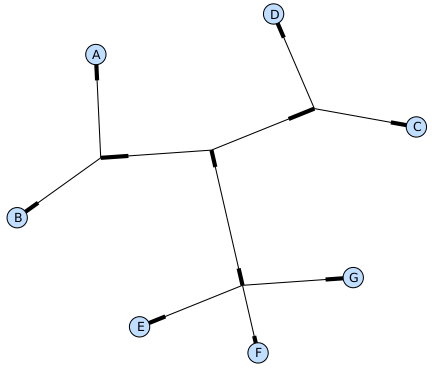
\includegraphics[width=0.45\textwidth]{images/phylo-rooted.png}
\caption{A rooted tree drawn with {\tt draw\_graphviz}.
Since we rooted the tree, we can see the root must be along the branch with two
directional ``heads''.
}
\label{fig:phylo-rooted}
\end{figure}
\begin{figure}[ptb]
\centering
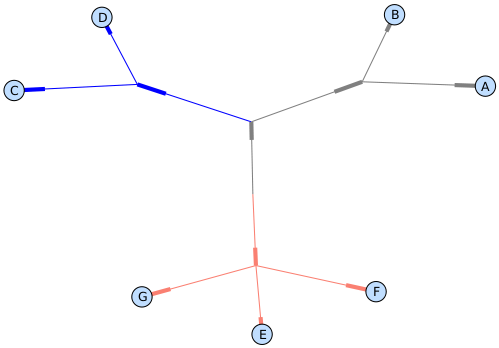
\includegraphics[width=0.5\textwidth]{images/phylo-color.png}
\caption{A colorized tree drawn with {\tt draw\_graphviz}, using {\tt neato} for node layout.}
\label{fig:phylo-color}
\end{figure}
\end{latexonly}

\begin{verbatim}
>>> Phylo.draw_graphviz(tree, prog="neato")
\end{verbatim}

\begin{htmlonly}
\imgsrc[width=499, height=348]{images/phylo-color.png}
\label{fig:phylo-color}
\end{htmlonly}

This viewing mode is particularly handy for exploring larger trees, because the matplotlib
viewer can zoom in on a selected region, thinning out a cluttered graphic.
\begin{latexonly}
%Can't reference unless inside a figure
(See Figs.~\ref{fig:phylo-apaf}, \ref{fig:phylo-apaf-zoom}).
\end{latexonly}

\begin{verbatim}
>>> tree = Phylo.read("apaf.xml", "phyloxml")
>>> Phylo.draw_graphviz(tree, prog="neato", node_size=0)
\end{verbatim}

\begin{htmlonly}
\imgsrc[width=519, height=400]{images/phylo-apaf.png}
\label{fig:phylo-apaf}
\imgsrc[width=506, height=400]{images/phylo-apaf-zoom.png}
\label{fig:phylo-apaf-zoom}
\end{htmlonly}

\begin{latexonly}
  \begin{figure}[tbp]
    \centering
    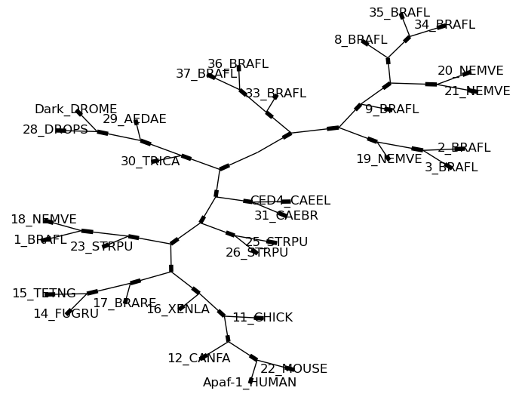
\includegraphics[width=0.65\textwidth]{images/phylo-apaf.png} \\
    \caption{A larger tree, using {\tt neato} for layout.}
    \label{fig:phylo-apaf}
  \end{figure}
  \begin{figure}[btp]
    \centering
    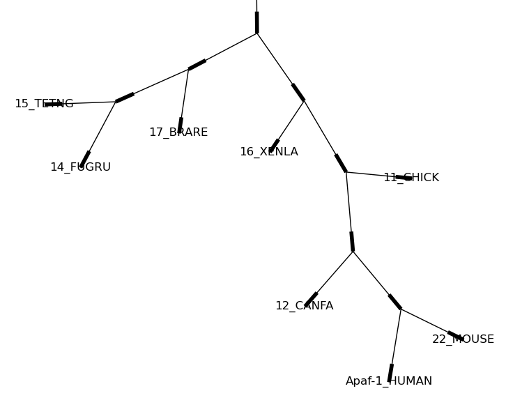
\includegraphics[width=0.6\textwidth]{images/phylo-apaf-zoom.png}
    \caption{A zoomed-in portion of the same tree as Fig.~\ref{fig:phylo-apaf}.}
    \label{fig:phylo-apaf-zoom}
  \end{figure}
\end{latexonly}

Note that branch lengths are not displayed accurately, because Graphviz ignores them when
creating the node layouts. The branch lengths are retained when exporting a tree as a NetworkX
graph object (\verb|to_networkx|), however.

See the Phylo page on the Biopython wiki (\url{http://biopython.org/wiki/Phylo}) for
descriptions and examples of the more advanced functionality in \verb|draw_ascii|,
\verb|draw_graphviz| and \verb|to_networkx|.


\section{Using Tree and Clade objects}

The \verb|Tree| objects produced by \verb|parse| and \verb|read| are containers for recursive
sub-trees, attached to the \verb|Tree| object at the \verb|root| attribute (whether or not the
phylogenic tree is actually considered rooted). A \verb|Tree| has globally applied information
for the phylogeny, such as rootedness, and a reference to a single \verb|Clade|; a
\verb|Clade| has node- and clade-specific information, such as branch length, and a list of
its own descendent \verb|Clade| instances, attached at the \verb|clades| attribute.

So there is a distinction between \verb|tree| and \verb|tree.root|. In practice, though, you
rarely need to worry about it. To smooth over the difference, both \verb|Tree| and
\verb|Clade| inherit from \verb|TreeMixin|, which contains the implementations for methods
that would be commonly used to search, inspect or modify a tree or any of its clades. This
means that almost all of the methods supported by \verb|tree| are also available on
\verb|tree.root| and any clade below it. (\verb|Clade| also has a \verb|root| property, which
returns the clade object itself.)

% TODO - use dia to make a class diagram like images/smcra.png

\subsection{Search and traversal methods}

For convenience, we provide a couple of simplified methods that return all external or internal
nodes directly as a list:

\begin{description}
  \item[\texttt{get\_terminals}] makes a list of all of this tree's terminal (leaf) nodes.
  \item[\texttt{get\_nonterminals}] makes a list of all of this tree's nonterminal (internal)
    nodes.
\end{description}

These both wrap a method with full control over tree traversal, \verb|find_clades|. Two more
traversal methods, \verb|find_elements| and \verb|find_any|, rely on the same core
functionality and accept the same arguments, which we'll call a ``target specification'' for
lack of a better description. These specify which objects in the tree will be matched and
returned during iteration. The first argument can be any of the following types:

\begin{itemize}
  \item A \textbf{TreeElement instance}, which tree elements will match by identity --- so
    searching with a Clade instance as the target will find that clade in the tree;

  \item A \textbf{string}, which matches tree elements' string representation --- in
    particular, a clade's \verb|name| \textit{(added in Biopython 1.56)};

  \item A \textbf{class} or \textbf{type}, where every tree element of the same type (or
    sub-type) will be matched;

  \item A \textbf{dictionary} where keys are tree element attributes and values are matched to the
    corresponding attribute of each tree element. This one gets even more elaborate:

    \begin{itemize}
      \item If an \texttt{int} is given, it matches numerically equal attributes, e.g. 1 will
        match 1 or 1.0

      \item If a boolean is given (True or False), the corresponding attribute value is
        evaluated as a boolean and checked for the same

      \item \texttt{None} matches \texttt{None}

      \item If a string is given, the value is treated as a regular expression (which must
        match the whole string in the corresponding element attribute, not just a prefix).  A
        given string without special regex characters will match string attributes exactly, so
        if you don't use regexes, don't worry about it.  For example, in a tree with clade
        names Foo1, Foo2 and Foo3, \verb|tree.find_clades({"name": "Foo1"})| matches Foo1,
        \verb|{"name": "Foo.*"}| matches all three clades, and \verb|{"name": "Foo"}| doesn't
        match anything.

    \end{itemize}

    Since floating-point arithmetic can produce some strange behavior, we don't support
    matching \texttt{float}s directly. Instead, use the boolean \texttt{True} to match every
    element with a nonzero value in the specified attribute, then filter on that attribute
    manually with an inequality (or exact number, if you like living dangerously).

    If the dictionary contains multiple entries, a matching element must match each of the
    given attribute values --- think ``and'', not ``or''.

  \item A \textbf{function} taking a single argument (it will be applied to each element in the
    tree), returning True or False. For convenience, LookupError, AttributeError and ValueError
    are silenced, so this provides another safe way to search for floating-point values in the
    tree, or some more complex characteristic.

\end{itemize}

After the target, there are two optional keyword arguments:

\begin{description}
  \item[terminal] --- A boolean value to select for or against terminal clades (a.k.a. leaf
    nodes): True searches for only terminal clades, False for non-terminal (internal) clades,
    and the default, None, searches both terminal and non-terminal clades, as well as any tree
    elements lacking the \verb|is_terminal| method.

  \item[order] --- Tree traversal order: \texttt{"preorder"} (default) is depth-first search,
    \texttt{"postorder"} is DFS with child nodes preceding parents, and \texttt{"level"} is
    breadth-first search.

\end{description}

Finally, the methods accept arbitrary keyword arguments which are treated the same way as a
dictionary target specification: keys indicate the name of the element attribute to search for,
and the argument value (string, integer, None or boolean) is compared to the value of each
attribute found. If no keyword arguments are given, then any TreeElement types are matched.
The code for this is generally shorter than passing a dictionary as the target specification:
\verb|tree.find_clades({"name": "Foo1"})| can be shortened to
\verb|tree.find_clades(name="Foo1")|.

(In Biopython 1.56 or later, this can be even shorter: \verb|tree.find_clades("Foo1")|)

% TODO -- introduce these / segue and clean up the descriptions

Now that we've mastered target specifications, here are the methods used to traverse a tree:

\begin{description}
  \item[\texttt{find\_clades}]
    Find each clade containing a matching element. That is, find each element as with
    \verb|find_elements|, but return the corresponding clade object. (This is usually what you
    want.)

    The result is an iterable through all matching objects, searching depth-first by default.
    This is not necessarily the same order as the elements appear in the Newick, Nexus or XML
    source file!

  \item[\texttt{find\_elements}]
    Find all tree elements matching the given attributes, and return the matching elements
    themselves. Simple Newick trees don't have complex sub-elements, so this behaves the same
    as \verb|find_clades| on them. PhyloXML trees often do have complex objects attached to
    clades, so this method is useful for extracting those.

  \item[\texttt{find\_any}]
    Return the first element found by \verb|find_elements()|, or None. This is also useful for
    checking whether any matching element exists in the tree, and can be used in a conditional.

\end{description}

Two more methods help navigating between nodes in the tree:

\begin{description}
  \item[\texttt{get\_path}]
    List the clades directly between the tree root (or current clade) and the given target.
    Returns a list of all clade objects along this path, ending with the given target, but
    excluding the root clade.

  \item[\texttt{trace}]
    List of all clade object between two targets in this tree. Excluding start, including
    finish.

\end{description}

\subsection{Information methods}

These methods provide information about the whole tree (or any clade).

\begin{description}
  \item[\texttt{common\_ancestor}]
    Find the most recent common ancestor of all the given targets. (This will be a Clade object).
    If no target is given, returns the root of the current clade (the one this method is called
    from); if 1 target is given, this returns the target itself.  However, if any of the
    specified targets are not found in the current tree (or clade), an exception is raised.

  \item[\texttt{count\_terminals}]
    Counts the number of terminal (leaf) nodes within the tree.

  \item[\texttt{depths}]
    Create a mapping of tree clades to depths. The result is a dictionary where the keys are
    all of the Clade instances in the tree, and the values are the distance from the root to
    each clade (including terminals). By default the distance is the cumulative branch length
    leading to the clade, but with the \verb|unit_branch_lengths=True| option, only the number
    of branches (levels in the tree) is counted.

  \item[\texttt{distance}]
    Calculate the sum of the branch lengths between two targets.  If only one target is
    specified, the other is the root of this tree.

  \item[\texttt{total\_branch\_length}]
    Calculate the sum of all the branch lengths in this tree. This is usually just called the
    ``length'' of the tree in phylogenetics, but we use a more explicit name to avoid confusion
    with Python terminology.

\end{description}

The rest of these methods are boolean checks:

\begin{description}
  \item[\texttt{is\_bifurcating}]
    True if the tree is strictly bifurcating; i.e. all nodes have either 2 or 0 children
    (internal or external, respectively). The root may have 3 descendents and still be
    considered part of a bifurcating tree.

  \item[\texttt{is\_monophyletic}]
    Test if all of the given targets comprise a complete subclade --- i.e., there
    exists a clade such that its terminals are the same set as the given targets. The targets
    should be terminals of the tree. For convenience, this method returns the common ancestor
    (MCRA) of the targets if they are monophyletic (instead of the value \verb|True|), and
    \verb|False| otherwise.

  \item[\texttt{is\_parent\_of}] True if target is a descendent of this tree --- not required
    to be a direct descendent. To check direct descendents of a clade, simply use list
    membership testing: \verb|if subclade in clade: ...|

  \item[\texttt{is\_preterminal}] True if all direct descendents are terminal; False if any
    direct descendent is not terminal.

\end{description}


\subsection{Modification methods}

These methods modify the tree in-place. If you want to keep the original tree intact, make a
complete copy of the tree first, using Python's \texttt{copy} module:

\begin{verbatim}
tree = Phylo.read('example.xml', 'phyloxml')
import copy
newtree = copy.deepcopy(tree)
\end{verbatim}

\begin{description}
  \item[\texttt{collapse}]
    Deletes the target from the tree, relinking its children to its parent.

  \item[\texttt{collapse\_all}]
    Collapse all the descendents of this tree, leaving only terminals. Branch lengths are
    preserved, i.e. the distance to each terminal stays the same. With a target specification
    (see above), collapses only the internal nodes matching the specification.

  \item[\texttt{ladderize}]
    Sort clades in-place according to the number of terminal nodes.  Deepest clades are placed
    last by default. Use \verb|reverse=True| to sort clades deepest-to-shallowest.

  \item[\texttt{prune}]
    Prunes a terminal clade from the tree.  If taxon is from a bifurcation, the connecting node
    will be collapsed and its branch length added to remaining terminal node. This might no
    longer be a meaningful value.

  \item[\texttt{root\_with\_outgroup}]
    Reroot this tree with the outgroup clade containing the given targets, i.e. the common
    ancestor of the outgroup. This method is only available on Tree objects, not Clades.

    If the outgroup is identical to self.root, no change occurs. If the outgroup clade is
    terminal (e.g. a single terminal node is given as the outgroup), a new bifurcating root
    clade is created with a 0-length branch to the given outgroup. Otherwise, the internal node
    at the base of the outgroup becomes a trifurcating root for the whole tree. If the original
    root was bifurcating, it is dropped from the tree.

    In all cases, the total branch length of the tree stays the same.

  \item[\texttt{root\_at\_midpoint}]
    Reroot this tree at the calculated midpoint between the two most distant
    tips of the tree. (This uses \verb|root_with_outgroup| under the hood.)

  \item[\texttt{split}]
    Generate \textit{n} (default 2) new descendants. In a species tree, this is a speciation
    event.  New clades have the given \verb|branch_length| and the same name as this clade's
    root plus an integer suffix (counting from 0) --- for example, splitting a clade named
    ``A'' produces the sub-clades ``A0'' and ``A1''.

\end{description}

See the Phylo page on the Biopython wiki (\url{http://biopython.org/wiki/Phylo}) for
more examples of using the available methods.


\subsection{Features of PhyloXML trees}
\label{sec:PhyloXML}

The phyloXML file format includes fields for annotating trees with additional data types and
visual cues.

% TODO
% annotations -- see wiki and epydoc pages
%     - on wiki, discuss each class

See the PhyloXML page on the Biopython wiki (\url{http://biopython.org/wiki/PhyloXML}) for
descriptions and examples of using the additional annotation features provided by PhyloXML.


% The object hierarchy still looks and behaves similarly:

% \begin{verbatim}
% >>> print(tree)

% Phylogeny(rooted=True, name="")
%     Clade(branch_length=1.0)
%         Clade(branch_length=1.0)
%             Clade(branch_length=1.0)
%                 Clade(branch_length=1.0, name="A")
%                 Clade(branch_length=1.0, name="B")
%             Clade(branch_length=1.0)
%                 Clade(branch_length=1.0, name="C")
%                 Clade(branch_length=1.0, name="D")
%         Clade(branch_length=1.0)
%             Clade(branch_length=1.0, name="E")
%             Clade(branch_length=1.0, name="F")
%             Clade(branch_length=1.0, name="G")
% \end{verbatim}

\section{Running external applications}
\label{sec:PhyloApps}

While Bio.Phylo doesn't infer trees from alignments itself, there are third-party
programs available that do. These are supported through the module
\texttt{Bio.Phylo.Applications}, using the same general framework as
\texttt{Bio.Emboss.Applications}, \texttt{Bio.Align.Applications} and others.

Biopython 1.58 introduced a wrapper for PhyML
(\url{http://www.atgc-montpellier.fr/phyml/}). The program accepts an input alignment in
\texttt{phylip-relaxed} format (that's Phylip format, but without the 10-character limit
on taxon names) and a variety of options. A quick example:

\begin{verbatim}
>>> from Bio import Phylo
>>> from Bio.Phylo.Applications import PhymlCommandline
>>> cmd = PhymlCommandline(input='Tests/Phylip/random.phy')
>>> out_log, err_log = cmd()
\end{verbatim}

This generates a tree file and a stats file with the names
[\textit{input~filename}]\verb|_phyml_tree.txt| and
[\textit{input~filename}]\verb|_phyml_stats.txt|. The tree file is in Newick format:

\begin{verbatim}
>>> tree = Phylo.read('Tests/Phylip/random.phy_phyml_tree.txt', 'newick')
>>> Phylo.draw_ascii(tree)
\end{verbatim}

A similar wrapper for RAxML (\url{http://sco.h-its.org/exelixis/software.html})
was added in Biopython 1.60, and FastTree
(\url{http://www.microbesonline.org/fasttree/}) in Biopython 1.62.

Note that some popular Phylip programs, including \texttt{dnaml} and \texttt{protml},
are already available through the EMBOSS wrappers in \texttt{Bio.Emboss.Applications} if
you have the Phylip extensions to EMBOSS installed on your system.
See Section~\ref{sec:alignment-tools} for some examples and clues on how to use
programs like these.


\section{PAML integration}
\label{sec:PhyloPAML}

Biopython 1.58 brought support for PAML
(\url{http://abacus.gene.ucl.ac.uk/software/paml.html}), a suite of programs for
phylogenetic analysis by maximum likelihood. Currently the programs codeml, baseml and
yn00 are implemented. Due to PAML's usage of control files rather than command line
arguments to control runtime options, usage of this wrapper strays from the format of
other application wrappers in Biopython.

A typical workflow would be to initialize a PAML object, specifying an alignment file, a
tree file, an output file and a working directory. Next, runtime options are set via the
\texttt{set\_options()} method or by reading an existing control file. Finally, the
program is run via the \texttt{run()} method and the output file is automatically parsed
to a results dictionary.

Here is an example of typical usage of codeml:
\begin{verbatim}
>>> from Bio.Phylo.PAML import codeml
>>> cml = codeml.Codeml()
>>> cml.alignment = "Tests/PAML/alignment.phylip"
>>> cml.tree = "Tests/PAML/species.tree"
>>> cml.out_file = "results.out"
>>> cml.working_dir = "./scratch"
>>> cml.set_options(seqtype=1,
...         verbose=0,
...         noisy=0,
...         RateAncestor=0,
...         model=0,
...         NSsites=[0, 1, 2],
...         CodonFreq=2,
...         cleandata=1,
...         fix_alpha=1,
...         kappa=4.54006)
>>> results = cml.run()
>>> ns_sites = results.get("NSsites")
>>> m0 = ns_sites.get(0)
>>> m0_params = m0.get("parameters")
>>> print(m0_params.get("omega"))
\end{verbatim}

Existing output files may be parsed as well using a module's \texttt{read()} function:
\begin{verbatim}
>>> results = codeml.read("Tests/PAML/Results/codeml/codeml_NSsites_all.out")
>>> print(results.get("lnL max"))
\end{verbatim}

Detailed documentation for this new module currently lives on the Biopython wiki:
\url{http://biopython.org/wiki/PAML}

\section{Future plans}
\label{sec:PhyloFuture}

Bio.Phylo is under active development. Here are some features we might add in future
releases:

\begin{description}
  \item[New methods]
    Generally useful functions for operating on Tree or Clade objects appear on the Biopython
    wiki first, so that casual users can test them and decide if they're useful before we add
    them to Bio.Phylo:

    \url{http://biopython.org/wiki/Phylo_cookbook}

  \item[Bio.Nexus port]
    Much of this module was written during Google Summer of Code 2009, under the auspices of
    NESCent, as a project to implement Python support for the phyloXML data format (see
    \ref{sec:PhyloXML}). Support for Newick and Nexus formats was added by porting part of the
    existing Bio.Nexus module to the new classes used by Bio.Phylo.

    Currently, Bio.Nexus contains some useful features that have not yet been ported to
    Bio.Phylo classes --- notably, calculating a consensus tree. If you find some functionality
    lacking in Bio.Phylo, try poking throught Bio.Nexus to see if it's there instead.

\end{description}

We're open to any suggestions for improving the functionality and usability of this module;
just let us know on the mailing list or our bug database.

Finally, if you need additional functionality not yet included in the Phylo
module, check if it's available in another of the high-quality Python libraries
for phylogenetics such as DendroPy (\url{http://pythonhosted.org/DendroPy/}) or
PyCogent (\url{http://pycogent.org/}). Since these libraries also support
standard file formats for phylogenetic trees, you can easily transfer data
between libraries by writing to a temporary file or StringIO object.


